\documentclass[a4paper, 11pt]{beamer}

\usepackage[utf8]{inputenc}
\usepackage[T1]{fontenc}
\usepackage{changepage}

\author{Jules Kozolinsky}
\title{Documentation, tests and others useful software engineering tools }
\date{}
\institute{ENS Paris-Saclay}

\usetheme{Hannover}
\usecolortheme{whale}

\setbeamertemplate{navigation symbols}{
    \usebeamerfont{footline}
    \usebeamercolor[fg]{footline}
    \hspace{1em}
    \insertframenumber/\inserttotalframenumber
}

\AtBeginSection[]{
    \begin{frame}
        \frametitle{Contents}
        \tableofcontents[currentsection]
    \end{frame}
}

\begin{document}

\begin{frame}
    \titlepage
\end{frame}

\section*{Introduction}

\begin{frame}
    \frametitle{\secname~: Different SWE tools}
    \begin{itemize}
        \item Git (via GitHub)
        \item Convention (pylint)
        \item Documentation (doxygen)
        \item Test (Travis, Unittest)
    \end{itemize}
\end{frame}

\section{Git}

\begin{frame}
    \frametitle{\secname~: Utilisation of Git}
    \begin{itemize}
        \item version control system (commits)
        \item different branches 
        \item decentralized
    \end{itemize}
\end{frame}

\begin{frame}
    \frametitle{\secname~: Utilisation of GitHub}
    Why ?
    \begin{itemize}
        \item simple to use
        \item issues
        \item compatible with continuous integration tools 
        \item nice graphs 
    \end{itemize}
\end{frame}

\begin{frame}
    \frametitle{\secname}
    \begin{itemize}
    	\item \textit{https://github.com/mkRPGDev/mkRPG}
        \item $16$ issues
        \item $\simeq 600$ commits
        \item $17$ branches whose one for documentation
    \end{itemize}
\end{frame}

\section{Convention}
\begin{frame}
    \frametitle{\secname~: \href{https://www.python.org/dev/peps/pep-0008/}{PEP 8 -- Style Guide for Python Code}}
    \begin{itemize}
        \item code lay-out
        \item whitespace in expressions and statements
        \item documentation strings
        \item naming conventions
    \end{itemize}
\end{frame}

\begin{frame}
    \frametitle{\secname~: Pylint - enforce coding standard}
    \begin{itemize}
        \item errors and warning
        \item statistics and note 
        \item different format
        \item pre-commit hook 
    \end{itemize}  
    Our code : $5.09/10$
\end{frame}

\section{Documentation}
\begin{frame}
    \frametitle{\secname~: Why ?}
    \begin{itemize}
        \item readable for the writer
        \item understandable by others 
        \item easy debug
    \end{itemize}
\end{frame}

\begin{frame}
    \frametitle{\secname~: Doxygen}
    Documentation generated by doxygen
    \begin{itemize}
    	\item automatically generated
        \item html or tex
        \item nice graphs
    \end{itemize}
\end{frame}

\begin{frame}
    \frametitle{\secname~: Doxygen}
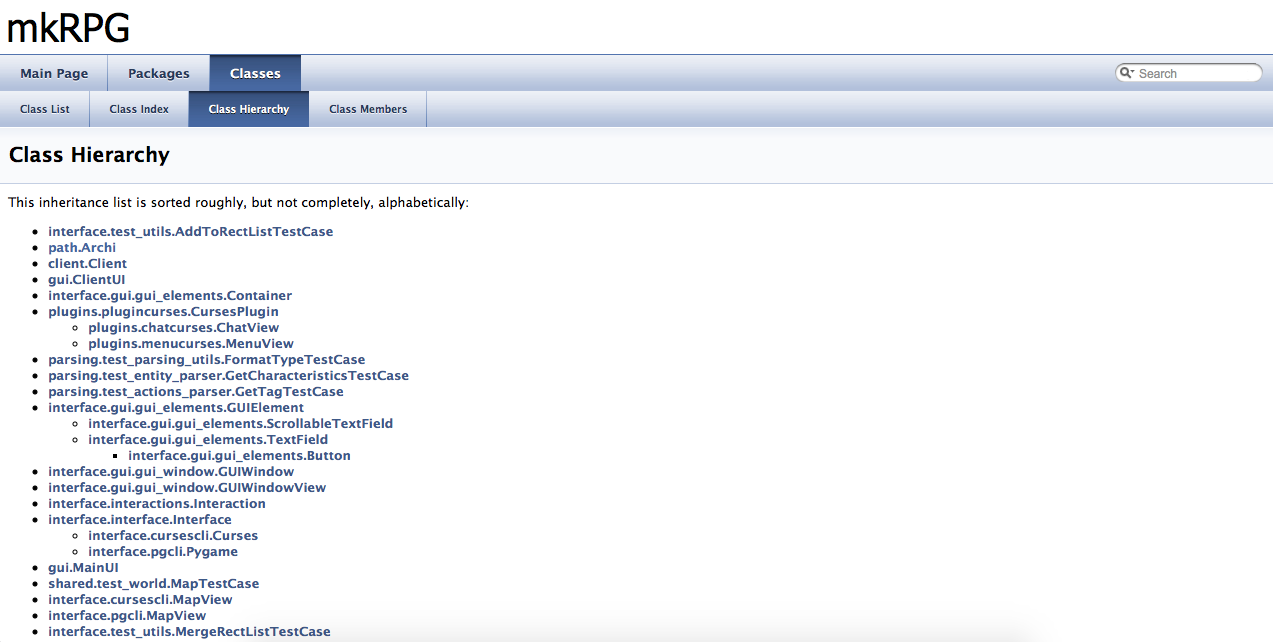
\includegraphics[scale=0.3]{doxygen}
\end{frame}

\section{Tests}
\begin{frame}
    \frametitle{\secname~}
    \begin{itemize}
    	\item \textit{"There ARE bugs in your code."}
        \item Static analysis (pylint)
        \item Unit testing (unittest)
    \end{itemize}
\end{frame}

\subsection{Unit testing}
\begin{frame}
    \frametitle{\secname~: Unittest}
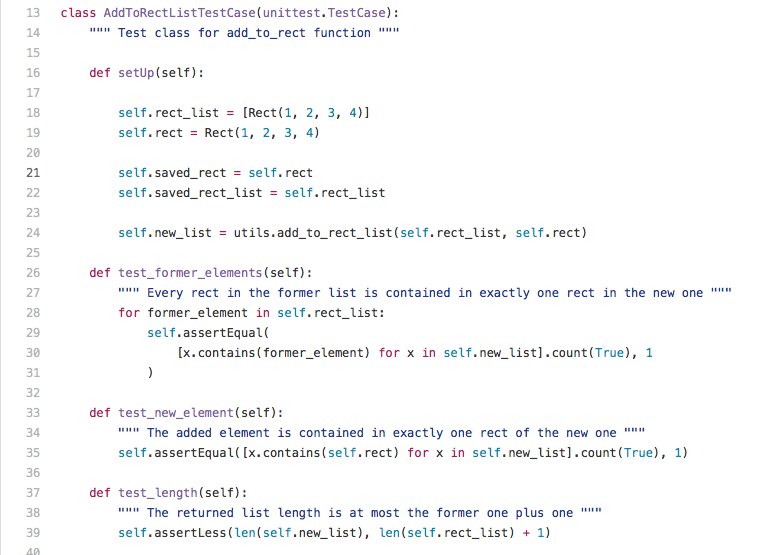
\includegraphics[scale=0.4]{unittest}
\end{frame}

\subsection{Continuons Integration}
\begin{frame}
    \frametitle{\secname~: Travis}
    Every modification of code runs code on server to check if anything bad happend
    \begin{itemize}
    	 \item Unittest (unit testing)
        \item Doxygen (documentation)
        \item Pylint (static code analysis)
    \end{itemize}
\end{frame}

\begin{frame}
    \frametitle{\secname~: Travis}
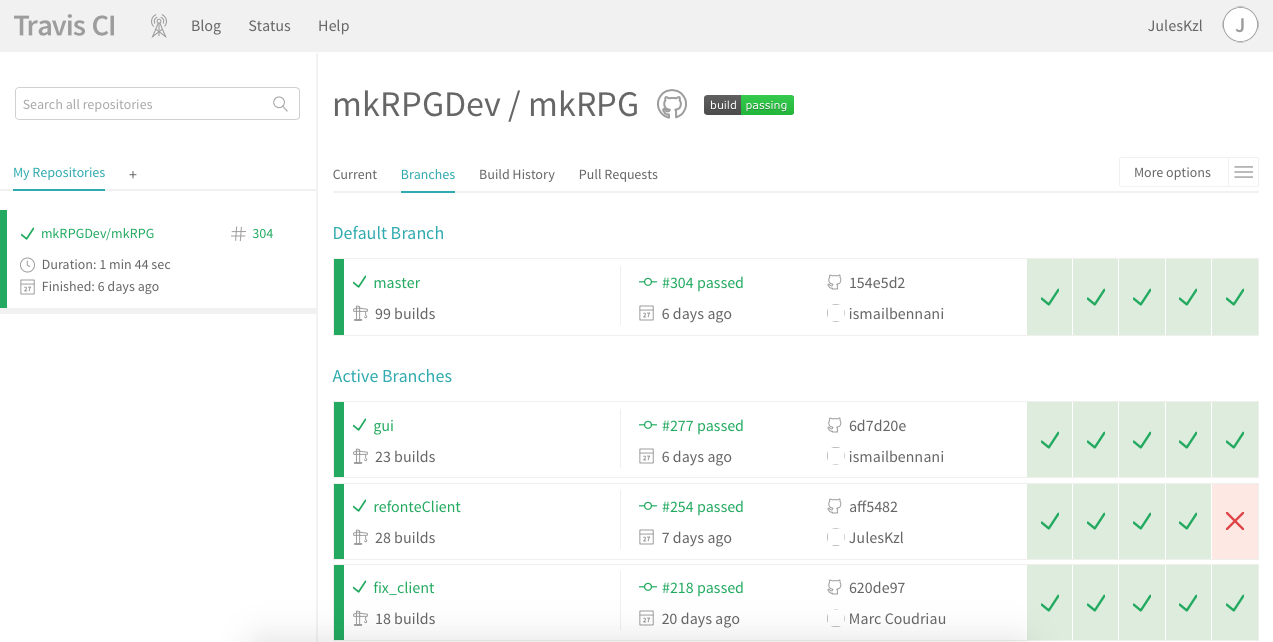
\includegraphics[scale=0.3]{travis}
\end{frame}



\end{document}
